\documentclass[11pt]{beamer}
\usetheme{Madrid}
\usepackage[utf8]{inputenc}
\usepackage{amsmath}
\usepackage{amsfonts}
\usepackage{amssymb}
\usepackage{graphicx}
\usepackage{xcolor}
\usepackage{tikz}
\usepackage{geometry}
\usepackage{array}
\usepackage{longtable}

\title{EB2-NIW Post-Denial Strategy}
\subtitle{Master-Class Post-Adjudication Framework \& Strategic Litigation Tactics}
\author{Advanced Post-Adjudication Litigation Training System for the Long Game}
\date{\today}

\setbeamercovered{transparent}
\setbeamertemplate{navigation symbols}{}
\setbeamerfont{itemize/enumerate body}{size=\scriptsize}
\setbeamerfont{itemize/enumerate subbody}{size=\tiny}
\setbeamerfont{block body}{size=\scriptsize}
\setbeamerfont{block title}{size=\normalsize}

\begin{document}
	
	% TITLE SLIDE
	\begin{frame}
		\titlepage
		\centering
		\scriptsize \textit{What to Do After a USCIS Denial: The Complete Post-Denial Workflow}
	\end{frame}
	
	% ============================================================
	% SECTION: INTRODUCTION
	% ============================================================
	
	\begin{frame}{What This Course Is (And Is Not)}
		\scriptsize
		\begin{block}{Course Expectations}
			\textbf{What This Course IS:}
			\begin{itemize}
				\item A strategic framework for navigating post-denial procedures
				\item A step-by-step system for filing MTR, MTC, FOIA, Mandamus, and APA
				\item A toolkit for pro se litigants to exhaust administrative remedies
				\item A roadmap to force government settlement and approval
			\end{itemize}
			\textbf{What This Course IS NOT:}
			\begin{itemize}
				\item \textcolor{red}{Legal advice} (I am not an attorney)
				\item \textcolor{red}{A guarantee of approval} (each case is unique)
				\item \textcolor{red}{A substitute for an immigration lawyer} (complex cases need attorneys)
				\item \textcolor{red}{A promise to overturn any denial} (results vary by case strength)
			\end{itemize}
		\end{block}
	\end{frame}
	
	
	% ============================================================
	% COMPLETE COURSE SECTIONS SUMMARY SLIDE
	% ============================================================
	
% ============================================================
% COMPLETE COURSE SECTIONS SUMMARY SLIDE (FONT REDUCED)
% ============================================================

\begin{frame}{Complete Course Sections Overview}
	\setbeamerfont{itemize/enumerate body}{size=\tiny}
	\setbeamerfont{itemize/enumerate subbody}{size=\tiny}
	\setbeamerfont{block body}{size=\tiny}
	\begin{block}{What This Course Covers - All Topics}
		\scriptsize
		\begin{columns}[T]
			\column{0.38\textwidth}
			\textbf{Section 1: Introduction \& Expectations}
			\tiny
			\begin{itemize}
				\item What this course is (and is NOT)
			 The "Long Game" concept
				 Realistic expectations
			\end{itemize}
			
			\textbf{Section 2: Understanding EB2-NIW Denials}
			\tiny
			\begin{itemize}
				\item Dhanasar 3 prongs explained
				Legal errors vs. factual disagreement
			 Why denials are "sticky"
			 RFE vs. NOID vs. Absolute Denial
			\end{itemize}
			
			\textbf{Section 3: The Correct 6-Step Sequence}
			\tiny
			\begin{itemize}
				\item MTR $\rightarrow$ Mandamus $\rightarrow$ MTC $\rightarrow$ Pre-Litigation $\rightarrow$ APA
			Flowchart visualization
			What each step does (and does NOT do)
			\end{itemize}
			
			\textbf{Section 4: Motion to Reopen (MTR)}
			\tiny
			\begin{itemize}
				\item Legal standard (8 C.F.R. § 103.5(a)(2))
			 The "Commitment Mistake"
				Katigbak rule - what's allowed vs. prohibited
			Clarifying expert letters strategy
				 MTR package structure
			\end{itemize}
			
			\textbf{Section 5: Motion to Reconsider (MTC)}
			\tiny
			\begin{itemize}
				\item Legal standard (8 C.F.R. § 103.5(a)(3))
				 Common legal errors to challenge
				 MTR vs. MTC decision matrix
			Combined MTR/MTC strategy
			\end{itemize}
			
			\column{0.58\textwidth}
			\textbf{Section 6: FOIA Strategy}
			\tiny
			\begin{itemize}
				\item What FOIA reveals about your denial
				 Internal documents you can obtain
			FOIA request template
			\end{itemize}
			
			\textbf{Section 7: Mandamus (Delay Strategy)}
			\tiny
			\begin{itemize}
				\item What Mandamus does (force decision, not approval)
				 When delay becomes actionable (6+ months)
				 Real case example (Texas)
			\end{itemize}
			
			\textbf{Section 8: APA Federal Lawsuit}
			\tiny
			\begin{itemize}
				\item When to file (ONLY at the very end)
			 Standard of review (arbitrary and capricious)
			 Complaint structure
				Prayer for relief template
			\end{itemize}
			
			\textbf{Section 9: Why You Must BLOCK AAO \& Voluntary Remand}
			\tiny
			\begin{itemize}
				\item AAO gives government new denial reasons
				 Voluntary remand gives another chance to deny
			 Cumulative error problem
				 How Pre-Litigation Notice blocks remand
			\end{itemize}
			
			\textbf{Section 10: Complete Case Walkthrough}
			\tiny
			\begin{itemize}
				\item Real timeline (denial $\rightarrow$ MTR $\rightarrow$ Mandamus $\rightarrow$ MTC $\rightarrow$ Pre-Litigation $\rightarrow$ APA $\rightarrow$ Approval)
			\end{itemize}
			
			\textbf{Section 11: Decision Matrix \& Error Avoidance}
			\tiny
			\begin{itemize}
				\item Common mistakes that destroy cases
			 Additional fatal errors
			 Quick reference charts (deadlines, fees, addresses)
			\end{itemize}
			
			\textbf{Section 12: Final Strategy Blueprint}
			\tiny
			\begin{itemize}
				\item Key Strategic Options (withdraw MTR)
			 Two paths to APA
				\item Final checklists and closing remarks
			\end{itemize}
		\end{columns}
	\end{block}
\end{frame}
	
	\begin{frame}{The "Long Game" Concept}
		\scriptsize
		\begin{block}{Why Denial $\neq$ End of Your Case}
			\textbf{Why denial is NOT the end:}
			\begin{itemize}
				\item Most denials contain legal errors that can be challenged
				\item USCIS officers are generalists who make mistakes
				\item The law provides multiple avenues for appeal and reconsideration
				\item Federal courts can review arbitrary agency actions
			\end{itemize}
			\textbf{Overview of the Full Path:}
			\begin{enumerate}
				\item Denial $\rightarrow$ MTR (30 days)
				\item FOIA (immediately) - get internal records
				\item Mandamus (if MTR delayed 6+ months)
				\item MTC (after MTR denied - 30 days)
				\item Pre-Litigation Notice (60 days)
				\item APA Complaint (final step)
				\item Government settles and approves (within 60 days of APA)
			\end{enumerate}
			\textcolor{blue}{The long game: 4-6 months from denial to approval if executed correctly.}
		\end{block}
	\end{frame}
	
	% ============================================================
	% SECTION: THE CORRECT SEQUENCE
	% ============================================================
	
	\begin{frame}{The Correct 6-Step Post-Denial Sequence}
		\scriptsize
		\begin{block}{The Master Sequence - APA ONLY at the VERY END}
			\textbf{Step 1:} Receive USCIS Denial
			\vspace{0.1cm}
			\textbf{Step 2:} File Motion to Reopen (MTR) within 30 days
			\vspace{0.1cm}
			\textbf{Step 3:} If USCIS delays MTR decision beyond 6 months $\rightarrow$ File Mandamus to force a decision on the MTR (NOT to challenge the denial)
			\vspace{0.1cm}
			\textbf{Step 4:} After USCIS denies MTR $\rightarrow$ File Motion to Reconsider (MTC) within 30 days
			\vspace{0.1cm}
			\textbf{Step 5:} After MTC denied $\rightarrow$ Send Pre-Litigation Notice (30-60 day warning to government)
			\vspace{0.1cm}
			\textbf{Step 6:} ONLY IF pre-litigation fails $\rightarrow$ File APA Complaint in Federal District Court (challenging the MTC denial as the final agency action if you have else MTR denial as the final agency action)
		\end{block}
	\end{frame}
	
	\begin{frame}{CRITICAL: APA Complaint is the LAST Resort}
		\scriptsize
		\begin{block}{What You DO NOT Do}
			\textcolor{red}{\textbf{NEVER file an APA Complaint challenging the original denial directly.}}
			\vspace{0.2cm}
			\textbf{Why not:}
			\begin{itemize}
				\item The original denial is NOT the final agency action if you filed an MTR and MTC
				\item Courts will dismiss for failure to exhaust administrative remedies
				\item You must give the agency every opportunity to correct its errors first
			\end{itemize}
		\end{block}
		\begin{block}{What You DO Instead}
			\textcolor{green}{\textbf{File APA Complaint ONLY after:}}
			\begin{enumerate}
				\item MTR filed and denied
				\item MTC filed and denied
				\item Pre-Litigation Notice sent and ignored
			\end{enumerate}
			\textbf{The APA Complaint challenges the MTC denial} (the final agency action after all administrative remedies exhausted).
		\end{block}
	\end{frame}
	
	\begin{frame}{The Correct Flowchart: APA at the VERY END}
		\scriptsize
		\begin{center}
			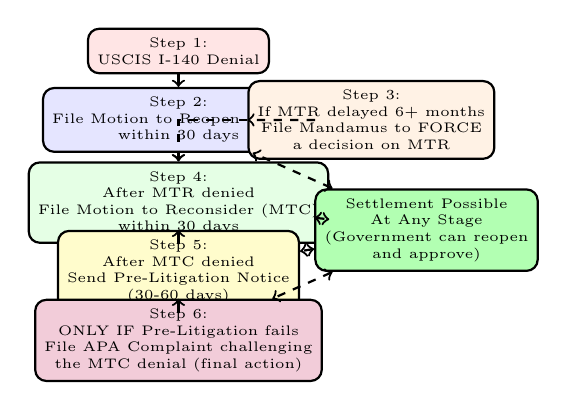
\begin{tikzpicture}[scale=0.35, every node/.style={draw, rounded corners, align=center, font=\tiny}]
				\node (denial) at (0,0) [fill=red!10, draw=black, thick] {Step 1:\\USCIS I-140 Denial};
				\node (mtr) at (0,-2.5) [fill=blue!10, draw=black, thick] {Step 2:\\File Motion to Reopen (MTR)\\within 30 days};
				\node (mandamus) at (7,-2.5) [fill=orange!10, draw=black, thick] {Step 3:\\If MTR delayed 6+ months\\File Mandamus to FORCE\\a decision on MTR};
				\node (mtc) at (0,-5.5) [fill=green!10, draw=black, thick] {Step 4:\\After MTR denied\\File Motion to Reconsider (MTC)\\within 30 days};
				\node (notice) at (0,-8) [fill=yellow!20, draw=black, thick] {Step 5:\\After MTC denied\\Send Pre-Litigation Notice\\(30-60 days)};
				\node (apa) at (0,-10.5) [fill=purple!20, draw=black, thick] {Step 6:\\ONLY IF Pre-Litigation fails\\File APA Complaint challenging\\the MTC denial (final action)};
				\node (settle) at (9,-6.5) [fill=green!30, draw=black, thick] {Settlement Possible\\At Any Stage\\(Government can reopen\\and approve)};
				
				\draw[->, thick] (denial) -- (mtr);
				\draw[->, thick] (mtr) -- (mtc);
				\draw[->, thick] (mtc) -- (notice);
				\draw[->, thick] (notice) -- (apa);
				\draw[->, dashed, thick] (mtr) -- (mandamus);
				\draw[->, dashed, thick] (mandamus) -| (mtc);
				\draw[<->, dashed, thick] (settle) -- (mtr);
				\draw[<->, dashed, thick] (settle) -- (mtc);
				\draw[<->, dashed, thick] (settle) -- (notice);
				\draw[<->, dashed, thick] (settle) -- (apa);
			\end{tikzpicture}
		\end{center}
	\end{frame}
	
	% ============================================================
	% SECTION: UNDERSTANDING DENIALS
	% ============================================================
	
	\begin{frame}{How USCIS Evaluates EB2-NIW (Dhanasar Three Prongs)}
		\scriptsize
		\begin{block}{Prong 1: The proposed endeavor has both substantial merit and national importance}
			\textbf{What USCIS Can Require:}
			\begin{itemize}
				\item The endeavor has broader implications beyond a single employer or location
				\item The endeavor impacts a field that is nationally significant (finance, AI, cybersecurity, healthcare, education)
				\item The endeavor has potential for future impact (prospective standard)
			\end{itemize}
			\textbf{What USCIS Cannot Require (Common Errors):}
			\begin{itemize}
				\item \textcolor{red}{Nationwide adoption or industry-wide transformation} (reserved for EB-1A)
				\item \textcolor{red}{Proof of immediate commercial success or revenue generation}
				\item \textcolor{red}{Letters from government agencies (though helpful, not required)}
				\item \textcolor{red}{Quantifiable metrics of already-demonstrated impact}
			\end{itemize}
		\end{block}
	\end{frame}
	
	\begin{frame}{Prong 2: Well-Positioned to Advance the Endeavor}
		\scriptsize
		\begin{block}{What USCIS Can Require:}
			\begin{itemize}
				\item Education, training, and experience in the field
				\item Progress toward the endeavor (preliminary work, publications, prototypes)
				\item Plan for executing the endeavor (timeline, milestones)
			\end{itemize}
			\textbf{What USCIS Cannot Require (Common Errors):}
			\begin{itemize}
				\item \textcolor{red}{A formal job offer or specific position title}
				\item \textcolor{red}{Proof that the endeavor has already succeeded}
				\item \textcolor{red}{Third-party funding or venture capital backing}
				\item \textcolor{red}{Employer sponsorship or institutional affiliation}
			\end{itemize}
			\textcolor{blue}{Self-petitioners are explicitly permitted under 8 C.F.R. § 204.5(k)(4)(ii).}
		\end{block}
	\end{frame}
	
	\begin{frame}{Prong 3: Balancing Test - Waiver Benefits the U.S.}
		\scriptsize
		\begin{block}{Factors Favoring a Waiver:}
			\begin{itemize}
				\item The endeavor is so urgent that waiting for labor certification would harm U.S. interests
				\item The nature of the work makes standard job testing impossible (e.g., self-employment, research, entrepreneurship)
				\item The petitioner has unique qualifications that cannot be easily replicated
			\end{itemize}
			\textbf{Common Misapplications:}
			\begin{itemize}
				\item \textcolor{red}{Requiring proof that no U.S. worker could perform the role}
				\item \textcolor{red}{Applying the PERM labor certification standard (different framework)}
				\item \textcolor{red}{Demanding employer sponsorship when self-petitioning}
			\end{itemize}
			\textcolor{blue}{The balancing test is the most subjective prong and often the easiest to challenge.}
		\end{block}
	\end{frame}
	
	\begin{frame}{The Psychology Behind a USCIS Denial}
		\scriptsize
		\begin{block}{Why Officers Deny When They Could Approve}
			\textbf{Understanding the adjudicator's mindset is critical to crafting an effective response:}
			\vspace{0.1cm}
			\begin{itemize}
				\item \textbf{Cover Your Tracks Culture:} Officers face internal audits. Denying a borderline case creates less professional risk than approving one that later gets flagged.
				\item \textbf{Template-Driven Denials:} Many denials use boilerplate language from previous cases. The officer may have applied a standard template without deeply analyzing your specific evidence.
				\item \textbf{Lack of Subject Matter Expertise:} Officers are generalists. They may not understand technical fields like quantitative finance, AI architecture, or specialized engineering.
				\item \textbf{Time Pressure:} Officers handle hundreds of files. They may spend 15-30 minutes on a petition that represents years of your work.
			\end{itemize}
			\textcolor{blue}{Understanding this psychology helps you write briefs that overcome their natural hesitation.}
		\end{block}
	\end{frame}
	
	\begin{frame}{The Difference Between Legal Error and Factual Disagreement}
		\scriptsize
		\begin{block}{Two Types of Denial Problems}
			\textbf{Legal Error (Winnable via MTC/APA):}
			\begin{itemize}
				\item Officer applied the wrong legal standard (e.g., required "field domination" for NIW)
				\item Officer ignored binding precedent (\textit{Dhanasar}, \textit{Chawathe})
				\item Officer considered factors forbidden by regulation
				\item Officer failed to provide reasoned explanation for rejecting evidence
			\end{itemize}
			\textbf{Factual Disagreement (Harder to Win):}
			\begin{itemize}
				\item Officer simply disagrees with your interpretation of the evidence
				\item Officer believes your evidence is insufficient (weight, not type)
				\item Officer questions your credibility or the credibility of your experts
			\end{itemize}
			\textcolor{red}{Legal errors are much easier to overturn than factual disagreements.}
		\end{block}
	\end{frame}
	
	\begin{frame}{Why Denials Are "Sticky" and Dangerous}
		\scriptsize
		\begin{block}{Collateral Consequences of a Denial}
			\textbf{1. Credibility Perception and History Tracking:}
			\begin{itemize}
				\item USCIS officers consistently retrieve historical petition patterns from internal databases before evaluating a new filing.
				\item A standing denial establishes an adverse baseline record, increasing psychological barriers for subsequent adjudicators.
			\end{itemize}
			\textbf{2. Parallel Filings / Future Category Adjustments:}
			\begin{itemize}
				\item Moving from an EB-2 NIW profile to an EB-1A profile post-denial signals an inconsistent evidentiary pivot to the center.
				\item Adjudicators scrutinize the sudden escalation from "national importance" to "extraordinary ability."
			\end{itemize}
			\textbf{3. Permanent Disclosure Mandates:}
			\begin{itemize}
				\item Statutory forms such as the I-485 Adjustment of Status and N-400 Naturalization explicitly require lifetime disclosure of all prior immigrant petition denials.
			\end{itemize}
		\end{block}
	\end{frame}
	
	\begin{frame}{Evidentiary Standings: Denial vs. RFE vs. NOID}
		\scriptsize
		\begin{block}{Structural Definitions under 8 C.F.R.}
			\centering
			\begin{tabular}{|p{3cm}|p{5cm}|p{2.5cm}|}
				\hline
				\textbf{Adjudicative Action} & \textbf{Procedural Meaning} & \textbf{Response Window} \\
				\hline
				RFE (Request for Evidence) & Core eligibility gaps found; administrative processing active. & 30 to 87 Days \\
				\hline
				NOID (Notice of Intent to Deny) & High-vulnerability stance; systemic defects that require structural remediation. & 30 to 33 Days \\
				\hline
				Absolute Denial & File is administratively closed; no further voluntary evidence is accepted. & 30 to 33 Days for initial legal action \\
				\hline
			\end{tabular}
			\vspace{0.2cm}
			\flushleft \textcolor{red}{\textbf{The Closed-Door Rule:}} Once an absolute denial is recorded, a service center will reject informal letters or supplemental evidence packages. To force them to look at your evidence, you must formally invoke an active jurisdictional remedy.
		\end{block}
	\end{frame}
	
	% ============================================================
	% SECTION: FOUNDATION BEFORE ACTION
	% ============================================================
	
	\begin{frame}{30-Day Rule \& Deadlines}
		\scriptsize
		\begin{block}{Critical Deadlines under 8 C.F.R. § 103.5(a)(1)(i)}
			\begin{itemize}
				\item The motion or appeal must be physically received by the designated USCIS intake facility within \textbf{30 days} of the exact decision date.
				\item The timeline scales to \textbf{33 days} if and only if the underlying denial notice was served on the applicant via standard, domestic US post.
			\end{itemize}
			\textcolor{red}{\textbf{No Equitable Tolling:}} Missing this window closes your path to local administrative remedies. If missed, your option is to file a fresh, baseline I-140 petition.
		\end{block}
	\end{frame}
	
	\begin{frame}{Choosing the Right Strategy}
		\scriptsize
		\begin{block}{MTR vs. MTC vs. AAO vs. Waiting}
			\centering
			\begin{tabular}{|p{4cm}|p{5cm}|}
				\hline
				\textbf{Strategy} & \textbf{When to Use} \\
				\hline
				MTR & New evidence available (clarifying expert letters, pre-filing documentation) \\
				\hline
				MTC & Legal error only, no new evidence needed \\
				\hline
				AAO & \textcolor{red}{AVOID} - gives government new denial reasons, no settlement authority \\
				\hline
				Waiting & Never - always act within 30 days \\
				\hline
			\end{tabular}
			\vspace{0.2cm}
			\textcolor{blue}{MTR is almost always the better first move. AAO is a trap.}
		\end{block}
	\end{frame}
	
	% ============================================================
	% SECTION: THE AAO PROBLEM
	% ============================================================
	
	\begin{frame}{Why AAO Appeals Have Low Success Rates}
		\scriptsize
		\begin{block}{Statistical Reality of Administrative Appeals}
			\textbf{Published AAO Data (Typical Year):}
			\begin{itemize}
				\item EB-1A/EB-2 NIW appeals: 85-90\% affirmed (denial sustained)
				\item 5-10\% remanded (sent back to service center for reconsideration)
				\item 2-5\% reversed (outright approval)
			\end{itemize}
			\textbf{Why AAO Affirms Most Denials:}
			\begin{itemize}
				\item Deferential standard of review (agency deference to its own officers)
				\item No new evidence permitted (you cannot fix gaps in the record)
				\item AAO is part of USCIS (institutional bias toward affirming)
				\item AAO lawyers are trained to find alternative grounds to sustain the denial
			\end{itemize}
			\textcolor{red}{Statistical reality: AAO is not designed to overturn denials; it is designed to review legal consistency.}
		\end{block}
	\end{frame}
	
	\begin{frame}{The AAO's Lack of Settlement Authority}
		\scriptsize
		\begin{block}{Why AAO Cannot Help You Negotiate}
			\textbf{What AAO Cannot Do:}
			\begin{itemize}
				\item Cannot engage in settlement discussions
				\item Cannot issue conditional approvals
				\item Cannot hold cases in abeyance for you to submit new evidence
				\item Cannot offer a "pathway to approval" with conditions
			\end{itemize}
			\textbf{What Federal Court Can Do:}
			\begin{itemize}
				\item DOJ attorneys have settlement authority
				\item Cases can be resolved via consent decree
				\item Government can voluntarily remand to service center with instructions to approve
				\item Your attorney can negotiate directly with government counsel
			\end{itemize}
			\textcolor{blue}{The AAO is a one-way door. Federal court is a two-way negotiation.}
		\end{block}
	\end{frame}
	
	\begin{frame}{The AAO vs. Local MTR: Strategic Comparison}
		\scriptsize
		\begin{block}{Decision Matrix for Choosing Your Path}
			\centering
			\begin{tabular}{|p{4cm}|p{3cm}|p{3cm}|}
				\hline
				\textbf{Factor} & \textbf{Local MTR} & \textbf{AAO Appeal} \\
				\hline
				New evidence allowed & YES & NO \\
				\hline
				Settlement possible & YES (with DOJ pressure) & NO \\
				\hline
				Timeline to decision & 3-6 months & 6-12+ months \\
				\hline
				Success rate (with strong evidence) & Moderate-High & Low \\
				\hline
				Preserves federal court option & YES & YES (after exhaustion) \\
				\hline
				Cost & Lower & Lower \\
				\hline
			\end{tabular}
			\vspace{0.2cm}
			\textcolor{blue}{MTR is almost always the better first move. AAO is a last resort.}
		\end{block}
	\end{frame}
	
	% ============================================================
	% SECTION: MOTION TO REOPEN (MTR)
	% ============================================================
	
	\begin{frame}{Motion to Reopen (MTR): Legal Architecture}
		\scriptsize
		\begin{block}{Regulatory Framework: 8 C.F.R. § 103.5(a)(2)}
			An MTR must satisfy a strict evidentiary threshold to be accepted by the local service center:
			\begin{enumerate}
				\item \textbf{Presentation of New, Material Facts:} Must articulate factual changes or clarifications that directly target the core of the denial.
				\item \textbf{Documentary Verification:} Must be supported by affidavits, newly rendered expert interpretation letters, or objective corporate documents.
				\item \textbf{The Discoverability Rule:} Must show that the evidence was not previously submitted to the record or readily discoverable during initial steps.
			\end{enumerate}
			\vspace{0.1cm}
			\textcolor{blue}{\textbf{Strategic Integration:}} Submitting clarifying expert evaluation letters through an MTR addresses the regulatory requirement locally while establishing a strong record for your Pre-Litigation file.
		\end{block}
	\end{frame}
	
	\begin{frame}{The "Commitment Mistake" in MTR Explained}
		\scriptsize
		\begin{block}{What Is the "Commitment Mistake"?}
			Many applicants file a Motion to Reopen without understanding a critical requirement:
			\vspace{0.2cm}
			\textcolor{red}{\textbf{You cannot file an MTR just because you disagree with the decision.}}
			\vspace{0.2cm}
			\textbf{The MTR Standard (8 C.F.R. § 103.5(a)(2)):}
			\begin{itemize}
				\item You must present \textbf{new, material facts}
				\item That were \textbf{not available and could not have been discovered} at the time of the original filing
				\item Supported by \textbf{affidavits or documentary evidence}
			\end{itemize}
			\textcolor{blue}{The "commitment mistake" is filing an MTR based only on legal disagreement, not on new facts.}
		\end{block}
	\end{frame}
	
	\begin{frame}{Commitment Mistake: Legal Disagreement vs. New Facts}
		\scriptsize
		\begin{block}{What USCIS Will Reject (Commitment Mistake)}
			\begin{quote}
				``I disagree with the officer's conclusion that my endeavor lacks national importance. The officer should have found that my work qualifies.''
			\end{quote}
			\textbf{Why this fails:} This is a legal disagreement, not a new fact. The officer already considered your evidence and disagreed.
			\vspace{0.3cm}
			\textbf{What USCIS Will Accept (Proper MTR):}
			\begin{quote}
				``New expert declaration (Exhibit A) from Dr. Smith, who was not available at the time of filing, confirms that my quantitative methodology was fully operational prior to the filing date. This new evidence directly addresses the officer's finding that the endeavor lacked operational capability.''
			\end{quote}
			\textcolor{green}{This is a new, material fact that existed but could not be presented earlier.}
		\end{block}
	\end{frame}
	
	\begin{frame}{When to File MTR vs. The Matter of Katigbak Trap}
		\scriptsize
		\begin{block}{Evaluating Your Evidentiary Posture}
			\textbf{Favorable Scenarios for an MTR:}
			\begin{itemize}
				\item Upgraded expert opinion letters explaining projects completed *prior* to your filing date.
				\item Hard copies of peer-reviewed indexing or university database profiles documenting your citation count exactly as it stood on the day you applied.
				\item Specialized blueprints or corporate deployment logs clarifying technical details the officer misread.
			\end{itemize}
			\textbf{The Fatal Flaw (\textit{Matter of Katigbak}, 14 I\&N Dec. 45):}
			\begin{itemize}
				\item \textcolor{red}{\textbf{You cannot use post-filing achievements.}} If you publish a new article, clear a new citation milestone, or receive a new award *after* your original filing date, it is legally barred from saving that specific petition.
			\end{itemize}
		\end{block}
	\end{frame}
	
	\begin{frame}{The Katigbak Rule Explained: What Is and Isn't Allowed}
		\scriptsize
		\begin{block}{\textit{Matter of Katigbak} (14 I\&N Dec. 45) - Key Holdings}
			\textbf{What Katigbak Prohibits:}
			\begin{itemize}
				\item Evidence of achievements that occurred \textbf{after} the filing date
				\item Post-filing publications, citations, awards, or job offers
				\item Any evidence that did not exist at the time of filing
			\end{itemize}
			\textbf{What Katigbak Does NOT Prohibit:}
			\begin{itemize}
				\item \textcolor{green}{Clarifying evidence about facts that existed at the time of filing}
				\item \textcolor{green}{Expert letters explaining why your pre-filing work has national importance}
				\item \textcolor{green}{Documentation of projects that were underway at filing}
				\item \textcolor{green}{Retrospective analysis of pre-filing achievements}
			\end{itemize}
			\textcolor{blue}{The distinction is between \textit{new facts} (not allowed) and \textit{clarifying explanations of existing facts} (allowed).}
		\end{block}
	\end{frame}
	
	\begin{frame}{Using the Clarifying Expert Letter to Bypass Katigbak}
		\scriptsize
		\begin{block}{Strategic Use of Post-Denial Expert Opinions}
			\textbf{Prohibited (Violates Katigbak):}
			\begin{quote}
				``Dr. Smith published a new paper in June 2025 (after denial) proving his methodology works.''
			\end{quote}
			\textbf{Permissible (Clarifies Existing Facts):}
			\begin{quote}
				``Dr. Smith's methodology, fully developed and operational as of March 2025 (before filing), has been independently reviewed by experts who confirm its national importance. Attached Exhibit A is a declaration from Dr. Jones explaining why the pre-existing methodology has broader implications for U.S. financial stability.''
			\end{quote}
			\textcolor{red}{The difference: You are not introducing new achievements. You are introducing \textit{expert interpretation} of achievements that already existed.}
		\end{block}
	\end{frame}
	
	\begin{frame}{Anatomy of an MTR Package}
		\scriptsize
		\begin{block}{Structural Filing Checklist for Local Service Centers}
			\begin{enumerate}
				\item \textbf{Form I-290B:} Executed with exact fee variations or authorized fee waiver documents.
				\item \textbf{Primary Cover Letter:} Formally detailing the requested local administrative actions.
				\item \textbf{Legal Brief:} Methodically proving that the newly introduced facts resolve the officer's doubts.
				\item \textbf{Indexed Exhibit Indexes:} Structured sequentially (Exhibit A-1, A-2, B-1...) to maximize readability under local file management conditions.
				\item \textbf{The Target Denial Notice:} A complete copy of the underlying adverse USCIS decision attached at the back of the brief.
			\end{enumerate}
			\vspace{0.1in}
			\textcolor{red}{\textbf{Logistical Rejection Notice:}} Minor clerical errors (missing a signature line or utilizing outdated fee rules) will cause an immediate rejection by the mailroom intake, wasting your 30-day window.
		\end{block}
	\end{frame}
	
	% ============================================================
	% SECTION: MOTION TO RECONSIDER (MTC)
	% ============================================================
	
	\begin{frame}{Motion to Reconsider (MTC): Legal Standard}
		\scriptsize
		\begin{block}{Regulatory Framework: 8 C.F.R. § 103.5(a)(3)}
			An MTC targets structural legal mistakes made by the adjudicating officer:
			\begin{enumerate}
				\item \textbf{Precise Legal Errors:} Must show exactly where the officer's analysis deviated from the law.
				\item \textbf{Binding Authority Alignment:} Must be supported by specific precedent decisions, statutory text, or federal regulations.
				\item \textbf{The Existing Record Rule:} Evaluated strictly on the file as it stood on decision day. **No new factual evidence, letters, or data points are allowed under an MTC.**
			\end{enumerate}
			\vspace{0.15cm}
			\textcolor{blue}{\textbf{The Combined Strategy:}} Select the option on Form I-290B for a \textbf{Combined Motion to Reopen and Reconsider (MTR/MTC)}. This allows you to introduce new clarifying expert letters while simultaneously addressing the officer's legal errors.
		\end{block}
	\end{frame}
	
	\begin{frame}{What MTC Does (and Does NOT Do)}
		\scriptsize
		\begin{block}{MTC is for Legal Errors, NOT New Evidence}
			\textbf{What MTC DOES:}
			\begin{itemize}
				\item Challenges legal errors in the original denial AND the MTR denial
				\item Argues the officer applied the wrong legal standard
				\item Cites binding precedent (\textit{Dhanasar}, \textit{Chawathe})
				\item Can be filed within 30 days of MTR denial
			\end{itemize}
			\textbf{What MTC DOES NOT Do:}
			\begin{itemize}
				\item \textcolor{red}{Cannot introduce new evidence (same record only)}
				\item \textcolor{red}{Cannot correct factual misunderstandings (use MTR for that)}
				\item \textcolor{red}{Cannot add post-filing achievements (Katigbak bar)}
			\end{itemize}
		\end{block}
	\end{frame}
	
	\begin{frame}{MTC Target: Common Legal Misapplications}
		\scriptsize
		\begin{block}{Exposing Systemic Violations in the I-140 Adjudication}
			\begin{enumerate}
				\item \textbf{The Heightened Standard Error:} Demanding proof of "field domination" or "immediate nationwide economic return" under the first prong of \textit{Matter of Dhanasar}. This illegally transforms a standard preponderance threshold into an EB-1A level hurdle.
				\item \textbf{Evidentiary Fragmentation:} Separating a cohesive, integrated analytical framework into isolated pieces, rather than evaluating its prospective impact holistically.
				\item \textbf{Arbitrary Expert Rejection:} Discounting authoritative opinion letters from industry leaders without providing a reasoned, fact-based justification in the record.
			\end{enumerate}
		\end{block}
	\end{frame}
	
	\begin{frame}{Additional Legal Errors to Challenge in an MTC}
		\scriptsize
		\begin{block}{More Common I-140 Adjudication Errors}
			\begin{enumerate}
				\item \textbf{The "Job Offer" Error:} Requiring a specific position title or employer when the NIW category explicitly permits self-petitioning (8 C.F.R. § 204.5(k)(4)(ii)).
				\item \textbf{The "Realized Impact" Error:} Demanding proof of already-demonstrated nationwide impact when \textit{Dhanasar} explicitly states the inquiry is "prospective."
				\item \textbf{The "Local Impact Only" Error:} Concluding that because the endeavor's primary impact is in one area, it lacks national importance, ignoring that broader implications can extend beyond that area.
				\item \textbf{The "Normal Job Duties" Error:} Reducing specialized, innovative work to "normal job duties" of a particular occupation without analyzing the specific endeavor.
				\item \textbf{The "Government Letter" Error:} Demanding formal government interest letters while ignoring actual government citations (Federal Reserve, Science.gov).
			\end{enumerate}
		\end{block}
	\end{frame}
	
	% ============================================================
	% SECTION: FOIA STRATEGY
	% ============================================================
	
	\begin{frame}{FOIA: Exposing the Internal Agency Mindset}
		\scriptsize
		\begin{block}{Freedom of Information Act (5 U.S.C. § 552) Application}
			\textbf{Why FOIA is a Vital Tool for Your Pre-Litigation File:}
			\begin{itemize}
				\item Extracts internal adjudicator worksheets, supervisory log books, and specific metadata trails.
				\item Identifies whether the officer relied on boilerplate text or cut-and-pasted language from completely unrelated denials.
				\item Pinpoints exactly where the reviewer's attention faltered during internal routing.
			\end{itemize}
			\textcolor{blue}{\textbf{Procedural Action Item:}} Submit your FOIA request digitally via FIRST or the direct DHS portal immediately upon receiving a denial notice. This record forms the core of your federal court filing.
		\end{block}
	\end{frame}
	
	\begin{frame}{What FOIA Can Reveal About Your Denial}
		\scriptsize
		\begin{block}{Internal Documents You Can Obtain}
			\textbf{Adjudicator Worksheets:}
			\begin{itemize}
				\item The officer's checklist of eligibility criteria
				\item Notes on what evidence was reviewed
				\item Timestamps showing how long the officer spent on your case
			\end{itemize}
			\textbf{Supervisory Review Notes:}
			\begin{itemize}
				\item Comments from senior officers who reviewed the denial
				\item Instructions to the adjudicator on how to frame the denial
			\end{itemize}
			\textbf{Email Communications:}
			\begin{itemize}
				\item Internal emails discussing your case
				\item Requests for additional information between officers
			\end{itemize}
			\textbf{System Logs:}
			\begin{itemize}
				\item Dates when your file was accessed
				\item Which officers viewed your file and when
			\end{itemize}
			\textcolor{blue}{This information can reveal procedural errors or improper influences.}
		\end{block}
	\end{frame}
	
	\begin{frame}{FOIA Request Standard Text Template}
		\scriptsize
		\begin{block}{Sample Targeted Content for High-Skill Adjudication Files}
			\begin{quote}
				\scriptsize
				\textbf{FOIA Request -- Internal Adjudication Records for Form I-140}
				
				Pursuant to the Freedom of Information Act (5 U.S.C. § 552), I request immediate electronic access to the complete administrative record, including all internal notes, evaluator worksheets, supervisor review lines, and communication logs generated during the evaluation of Form I-140, Receipt Number [INSERT NUMBER], denied on [INSERT DATE]. 
				
				This request specifically targets the non-exempt internal adjudicator tracking metrics that show the explicit evaluation steps applied to the Petitioner's proposed endeavor.
			\end{quote}
		\end{block}
	\end{frame}
	
	% ============================================================
	% SECTION: MANDAMUS (DELAY STRATEGY)
	% ============================================================
	
	\begin{frame}{What Mandamus Does (and Does NOT Do)}
		\scriptsize
		\begin{block}{Mandamus is for DELAY, NOT for challenging the denial}
			\textbf{What Mandamus DOES:}
			\begin{itemize}
				\item Forces USCIS to issue a decision on your pending MTR
				\item Compels the agency to stop ignoring your case
				\item Gets your case moving after 6+ months of delay
				\item Can be filed in federal district court
			\end{itemize}
			\textbf{What Mandamus DOES NOT Do:}
			\begin{itemize}
				\item \textcolor{red}{Cannot tell USCIS to approve your MTR}
				\item \textcolor{red}{Cannot reverse the underlying denial}
				\item \textcolor{red}{Cannot challenge the substance of the denial}
				\item \textcolor{red}{Cannot substitute the court's judgment for the agency's}
			\end{itemize}
			\textcolor{blue}{Mandamus forces a decision - not a particular outcome. The decision could still be a denial.}
		\end{block}
	\end{frame}
	
	\begin{frame}{Why Mandamus Is Needed After MTR Filing}
		\scriptsize
		\begin{block}{The Mandamus Step: When USCIS Won't Decide}
			After you file a Motion to Reopen (MTR), USCIS may:
			\vspace{0.2cm}
			\begin{itemize}
				\item Sit on your motion for 6, 9, 12+ months
				\item Ignore your status inquiries
				\item Leave you in administrative limbo
			\end{itemize}
			\textbf{Without Mandamus:}
			\begin{itemize}
				\item You cannot move to the next step (MTC or federal court)
				\item Your case is stuck indefinitely
				\item USCIS has no legal obligation to decide quickly (no statutory deadline)
			\end{itemize}
			\textcolor{red}{Mandamus is the tool to force USCIS to issue a decision on your pending MTR.}
		\end{block}
	\end{frame}
	
	\begin{frame}{Mandamus Timeline: When to File}
		\scriptsize
		\begin{block}{Strategic Timing for Mandamus After MTR}
			\begin{tabular}{|p{3cm}|p{6cm}|}
				\hline
				\textbf{Time Since MTR Filing} & \textbf{Recommended Action} \\
				\hline
				0-3 months & Normal processing; wait \\
				\hline
				3-4 months & Send first status inquiry via phone/email \\
				\hline
				4-5 months & Send second status inquiry (written) \\
				\hline
				5-6 months & Send formal pre-mandamus notice to USCIS \\
				\hline
				6-8 months & File Mandamus complaint in federal court \\
				\hline
				8-12 months & Strong mandamus case (delay clearly unreasonable) \\
				\hline
				12+ months & Very strong mandamus case; likely to succeed \\
				\hline
			\end{tabular}
		\end{block}
	\end{frame}
	
	\begin{frame}{Mandamus: Example from Texas (NDTX)}
		\scriptsize
		\begin{block}{Case Example: Joshi v. Bondi et al. (NDTX 2026)}
			\textbf{Facts:}
			\begin{itemize}
				\item I-140 EB2-NIW denied August 29, 2025
				\item MTR filed September 21, 2025
				\item USCIS did not adjudicate MTR for 6+ months
				\item Filed Mandamus in Northern District of Texas
				\item USCIS responded by adjudicating MTR (denied, but acted)
			\end{itemize}
			\textbf{Result:}
			\begin{itemize}
				\item Mandamus compelled action
				\item USCIS could no longer delay
				\item Case dismissed as moot after action taken
			\end{itemize}
			\textcolor{blue}{Mandamus worked to force a decision - even if decision was negative.}
		\end{block}
	\end{frame}
	
	% ============================================================
	% SECTION: EXECUTING THE LITIGATION RUNWAY
	% ============================================================
	
	\begin{frame}{MTC: Challenge Both Denials}
		\scriptsize
		\begin{block}{Bundled Legal Challenges in MTC}
			Your Motion to Reconsider should challenge:
			\vspace{0.2cm}
			\textbf{Original I-140 Denial Errors:}
			\begin{itemize}
				\item Heightened standard error (field domination requirement)
				\item Evidentiary fragmentation
				\item Ignored expert opinion letters
				\item Prospective vs. realized impact confusion
			\end{itemize}
			\textbf{MTR Denial Errors:}
			\begin{itemize}
				\item Misapplication of \textit{Matter of Katigbak}
				\item Failure to recognize clarifying evidence as permissible
				\item Categorically rejecting new expert letters
				\item Arbitrary dismissal of pre-filing documentation
			\end{itemize}
			\textcolor{red}{A single MTC can (and should) challenge both denials simultaneously.}
		\end{block}
	\end{frame}
	
	\begin{frame}{Pre-Litigation Notice: What It Is}
		\scriptsize
		\begin{block}{Definition and Purpose}
			A Pre-Litigation Notice is a formal written communication sent to the government before filing a lawsuit.
			\vspace{0.2cm}
			\textbf{Purpose:}
			\begin{itemize}
				\item Notifies the government of your intent to sue
				\item Summarizes the legal errors in the agency's decisions
				\item Requests that the agency cure the errors within a specified timeframe
				\item Creates a record of good-faith effort to resolve without litigation
				\item Required by some courts before filing pro se
			\end{itemize}
			\textbf{Sent to:}
			\begin{itemize}
				\item DHS Secretary
				\item USCIS Director
				\item Service Center Director
				\item U.S. Attorney for your district
				\item Attorney General of the United States
			\end{itemize}
		\end{block}
	\end{frame}
	
	\begin{frame}{Why the Pre-Litigation Notice Works}
		\scriptsize
		\begin{block}{The Psychology of the Notice}
			\textbf{Why the government responds to pre-litigation notices:}
			\begin{itemize}
				\item \textbf{DOJ attorneys hate unnecessary lawsuits.} They would rather settle a clear case than spend months litigating.
				\item \textbf{Agencies have settlement authority.} USCIS can voluntarily reopen and approve a case without admitting error.
				\item \textbf{Court dockets are crowded.} Judges appreciate parties who try to resolve disputes before filing.
				\item \textbf{The notice creates a record.} If the government ignores the notice, that becomes evidence of bad faith in court.
			\end{itemize}
			\textcolor{blue}{A well-crafted pre-litigation notice is often sufficient to get a denial reopened without ever filing a lawsuit.}
		\end{block}
	\end{frame}
	
	\begin{frame}[allowframebreaks]{The Pre-Litigation Notice: Creating the Way Out}
		\scriptsize
		\begin{block}{Choreographing the Opportunity to Cure}
			Before filing a federal suit, send a formal \textbf{Pre-Litigation Notice and Opportunity to Cure} via USPS Certified Mail to the DHS Secretary, USCIS Director, and the local U.S. Attorney's Office.
			\vspace{0.15cm}
			\textbf{Core Elements of the Notice:}
			\begin{itemize}
				\item Identifies the precise violations of the Administrative Procedure Act (5 U.S.C. § 706) present in the MTC denial.
				\item States clearly that a Form I-290B Motion to Reconsider was filed and denied.
				\item Informs the government that if the error is not cured within a 30-to-60-day window, a federal lawsuit will be filed.
			\end{itemize}
		\end{block}
		\framebreak
		\begin{block}{Actual Language Template -- Demand and Notice}
			\begin{quote}
				``This letter serves as formal Pre-Litigation Notice and Opportunity to Cure regarding the arbitrary and capricious denial of the Petitioner's Motion to Reconsider. 
				
				The agency's reliance on extra-legal criteria violates the Administrative Procedure Act, 5 U.S.C. § 706. The Motion to Reconsider (filed [DATE]) was denied on [DATE]. 
				
				If the agency fails to exercise its authority to vacate the unlawful denial within forty-five (45) days, Plaintiff will initiate formal litigation in United States District Court seeking declaratory and injunctive relief against the MTC denial as the final agency action.''
			\end{quote}
		\end{block}
	\end{frame}
	
	% ============================================================
	% SECTION: APA COMPLAINT
	% ============================================================
	
	\begin{frame}{APA Complaint: Final Step After Pre-Litigation Fails}
		\scriptsize
		\begin{block}{When to File APA Complaint - ONLY at the VERY END}
			\textbf{Prerequisites before filing APA Complaint:}
			\begin{enumerate}
				\item MTR filed and denied
				\item MTC filed and denied
				\item Pre-Litigation Notice sent (30-60 days)
				\item Government ignored or refused to cure
			\end{enumerate}
			\textbf{What the APA Complaint challenges:}
			\begin{itemize}
				\item The MTC denial as the final agency action
				\item NOT the original denial (that is not final after MTR/MTC)
			\end{itemize}
		\end{block}
	\end{frame}
	
	\begin{frame}{What APA Complaint Does (Final Step Only)}
		\scriptsize
		\begin{block}{APA Complaint Challenges the MTC Denial as Final Agency Action}
			\textbf{What APA Complaint DOES:}
			\begin{itemize}
				\item Challenges the MTC denial as arbitrary, capricious, and contrary to law
				\item Asks the court to vacate the MTC denial and remand with instructions
				\item Filed ONLY after all administrative remedies exhausted
				\item Filed ONLY after pre-litigation notice ignored
			\end{itemize}
			\textbf{What APA Complaint DOES NOT Do:}
			\begin{itemize}
				\item \textcolor{red}{Cannot be filed directly against the original denial}
				\item \textcolor{red}{Cannot introduce new evidence (court reviews the record)}
				\item \textcolor{red}{Cannot be filed without exhausting MTR and MTC first}
			\end{itemize}
		\end{block}
	\end{frame}
	
	\begin{frame}{APA Litigation: Standard of Review}
		\scriptsize
		\begin{block}{How Courts Review Agency Decisions}
			\textbf{The Arbitrary and Capricious Standard (5 U.S.C. § 706(2)(A)):}
			\begin{itemize}
				\item Court asks: Did the agency articulate a rational connection between the facts found and the decision made?
				\item Did the agency consider all relevant factors?
				\item Did the agency ignore evidence that contradicted its conclusion?
				\item Did the agency provide a reasoned explanation for rejecting evidence?
			\end{itemize}
			\textbf{The Contrary to Law Standard (5 U.S.C. § 706(2)(B)):}
			\begin{itemize}
				\item Court asks: Did the agency apply the correct legal standard?
				\item Did the agency follow its own regulations and precedent?
				\item Did the agency exceed its statutory authority?
			\end{itemize}
			\textcolor{blue}{Courts give some deference to agencies, but not when they ignore their own regulations or binding precedent.}
		\end{block}
	\end{frame}
	
	\begin{frame}{APA Complaint Structure (Detailed)}
		\scriptsize
		\begin{block}{Required Sections for a Federal APA Complaint}
			\begin{enumerate}
				\item \textbf{Caption and Parties:} Plaintiff (you) vs. Federal Defendants (sued in official capacity)
				\item \textbf{Jurisdiction and Venue:} 28 U.S.C. § 1331 (federal question), 5 U.S.C. § 702 (APA), 28 U.S.C. § 1391(e) (venue for suits against officers)
				\item \textbf{Factual Background:} Chronological narrative of your case (filing, RFE, response, denial, MTR, MTR denial, MTC, MTC denial)
				\item \textbf{Administrative Exhaustion:} Statement that you have exhausted all administrative remedies (MTR and MTC filed and denied)
				\item \textbf{Legal Claims (Counts):} 
				\begin{itemize}
					\item Count 1: Violation of APA (arbitrary and capricious - MTC denial)
					\item Count 2: Violation of APA (contrary to law - MTC denial)
				\end{itemize}
				\item \textbf{Prayer for Relief:} Vacate MTC denial, remand with instructions
				\item \textbf{Exhibits:} Denial notices, MTR denial, MTC denial, Pre-Litigation Notice
			\end{enumerate}
		\end{block}
	\end{frame}
	
	\begin{frame}[allowframebreaks]{Actual Language Template -- APA Complaint Claims for Relief}
		\scriptsize
		\begin{block}{Unabridged Prayer for Relief (Final Step Only)}
			\begin{quote}
				WHEREFORE, Plaintiff respectfully requests that this Court:
				
				A. Declare that Defendant's denial of Plaintiff's Motion to Reconsider dated [MTC DENIAL DATE] is arbitrary, capricious, an abuse of discretion, and not in accordance with law under 5 U.S.C. § 706(2)(A);
				
				B. Declare that Defendant's denial of Plaintiff's Motion to Reconsider is contrary to law under 5 U.S.C. § 706(2)(B);
				
				C. Vacate the denial of Plaintiff's Motion to Reconsider (Receipt No. [NUMBER]);
				
				D. Remand this matter to USCIS for a lawful adjudication of the underlying Form I-140 EB-2 NIW petition consistent with \textit{Matter of Dhanasar}, 8 C.F.R. § 204.5(k), and the Administrative Procedure Act;
				
				E. Retain jurisdiction over this matter to ensure strict compliance with the Court's orders; and
				
				F. Grant such other and further relief as this Court deems just, equitable, and proper.
			\end{quote}
			\textcolor{red}{Note: The APA Complaint challenges the MTC denial, NOT the original I-140 denial.}
		\end{block}
	\end{frame}
	
	% ============================================================
	% SECTION: THE TRIAGE STRATEGY ARCHITECTURE
	% ============================================================
	
	\begin{frame}{The Triage Strategy Architecture}
		\scriptsize
		\begin{center}
			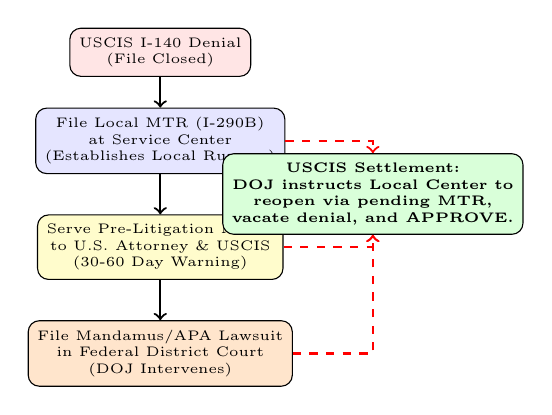
\begin{tikzpicture}[scale=0.45, every node/.style={draw, rounded corners, align=center, font=\tiny}]
				\node (denial) at (0,0) [fill=red!10] {USCIS I-140 Denial\\(File Closed)};
				\node (mtr) at (0,-2.5) [fill=blue!10] {File Local MTR (I-290B)\\at Service Center\\(Establishes Local Runway)};
				\node (notice) at (0,-5.5) [fill=yellow!20] {Serve Pre-Litigation Notice\\to U.S. Attorney \& USCIS\\(30-60 Day Warning)};
				\node (lawsuit) at (0,-8.5) [fill=orange!20] {File Mandamus/APA Lawsuit\\in Federal District Court\\(DOJ Intervenes)};
				\node (settle) at (6,-4) [fill=green!15, font=\bfseries\tiny] {USCIS Settlement:\\DOJ instructs Local Center to\\reopen via pending MTR,\\vacate denial, and APPROVE.};
				
				\draw[->, thick] (denial) -- (mtr);
				\draw[->, thick] (mtr) -- (notice);
				\draw[->, thick] (notice) -- (lawsuit);
				\draw[->, dashed, thick, red] (lawsuit) -| (settle);
				\draw[->, dashed, thick, red] (notice) -| (settle);
				\draw[->, dashed, thick, red] (mtr) -| (settle);
			\end{tikzpicture}
		\end{center}
	\end{frame}
	
	% ============================================================
	% SECTION: DECISION MATRIX & ERROR AVOIDANCE
	% ============================================================
	
	\begin{frame}{Decision Matrix: Selecting Your Path}
		\scriptsize
		\begin{block}{Remediation Framework Based on Evidentiary Posture}
			\centering
			\begin{tabular}{|p{4cm}|p{6.5cm}|}
				\hline
				\textbf{Evidentiary Posture} & \textbf{Prescribed Action Path} \\
				\hline
				New expert letters or filing-date metrics are available. & File a local \textbf{Motion to Reopen (MTR)} immediately to establish your settlement baseline. \\
				\hline
				Clear legal misapplication on the existing record with no new facts. & File a \textbf{Motion to Reconsider (MTC)} to challenge legal errors. \\
				\hline
			\end{tabular}
		\end{block}
	\end{frame}
	
	\begin{frame}{Decision Matrix: Timeline Posture}
		\scriptsize
		\begin{block}{Remediation Framework Based on Timeline Posture}
			\centering
			\begin{tabular}{|p{4cm}|p{6.5cm}|}
				\hline
				\textbf{Evidentiary Posture} & \textbf{Prescribed Action Path} \\
				\hline
				Local center refuses to rule or stalls the pending MTR for 6+ months. & Issue a formal \textbf{Mandamus} to force a decision on the MTR. \\
				\hline
				MTC denied and Pre-Litigation Notice ignored. & File \textbf{APA Complaint} challenging the MTC denial as final agency action. \\
				\hline
				Considering an AAO Appeal out of standard reflex. & \textbf{Avoid entirely.} The AAO has no out-of-court settlement authority and completely kills your local leverage. \\
				\hline
			\end{tabular}
		\end{block}
	\end{frame}
	
	\begin{frame}{Decision Matrix: Denial Type}
		\scriptsize
		\begin{block}{Remediation Framework Based on Denial Type}
			\centering
			\begin{tabular}{|p{4cm}|p{6.5cm}|}
				\hline
				\textbf{Denial Type} & \textbf{Prescribed Action Path} \\
				\hline
				Denial based on factual misunderstanding of your evidence. & \textbf{MTR with clarifying evidence.} Show the officer misread or missed key documents. \\
				\hline
				Denial based on legal error (wrong standard, misapplied precedent). & \textbf{MTC focusing on legal argument.} Cite \textit{Dhanasar}, Policy Manual, regulations. \\
				\hline
				Denial based on lack of evidence that you can now supply. & \textbf{Refile} (not appeal). MTR cannot introduce entirely new categories of evidence. \\
				\hline
				Denial that is clearly wrong on both facts and law. & \textbf{Combined MTR/MTC + Pre-Litigation Notice.} Apply maximum pressure. \\
				\hline
			\end{tabular}
		\end{block}
	\end{frame}
	
	\begin{frame}{Common Mistakes That Destroy Cases}
		\scriptsize
		\begin{block}{Fatal Post-Denial Mistakes to Avoid}
			\begin{enumerate}
				\item \textbf{Filing an AAO Appeal out of reflex:} This locks your case file in an appellate queue for months where local settlement is impossible.
				\item \textbf{Filing an MTC alone when you need to add new letters:} Because an MTC strictly forbids new facts, adding evidence causes an automatic, unappealable dismissal.
				\item \textbf{Filing an APA Complaint directly against the original denial:} Courts will dismiss for failure to exhaust administrative remedies.
				\item \textbf{Not exhausting MTR and MTC before APA:} The original denial is NOT the final agency action if you have pending motions.
			\end{enumerate}
		\end{block}
	\end{frame}
	
	\begin{frame}{Additional Common Mistakes to Avoid}
		\scriptsize
		\begin{block}{More Fatal Errors}
			\begin{enumerate}
				\item \textbf{Missing the 30-day deadline:} No extensions. If you miss it, your only option is to refile a new I-140.
				\item \textbf{Sending your MTR to the wrong address:} Different service centers handle different case types. Check USCIS website before mailing.
				\item \textbf{Using the wrong fee amount:} USCIS fees change periodically. Check the G-1055 fee schedule on the day you mail.
				\item \textbf{Forgetting to sign Form I-290B:} Unsigned forms are rejected immediately, and you may miss the deadline before resubmitting.
				\item \textbf{Not including proof of service:} You must show you served copies on all relevant government offices.
				\item \textbf{Filing without a legal brief:} Form I-290B alone is insufficient. You must attach a detailed legal argument.
				\item \textbf{Using emotional language:} Stick to facts, law, and evidence. Emotional appeals are ignored.
			\end{enumerate}
		\end{block}
	\end{frame}
	
	% ============================================================
	% SECTION: AI DRAFTING SYSTEM
	% ============================================================
	
	\begin{frame}{Using AI for MTR Drafting}
		\scriptsize
		\begin{block}{How AI Can Help Structure MTR Arguments}
			\textbf{AI can assist with:}
			\begin{itemize}
				\item Generate legal brief outlines based on your specific denial reasons
				\item Draft cover letters and exhibit indexes
				\item Summarize complex technical evidence for adjudicators
				\item Identify logical gaps in your argument
				\item Format citations and references correctly
			\end{itemize}
			\textbf{Example AI prompt for MTR:}
			\begin{quote}
				``Draft a Motion to Reopen legal brief arguing that new expert declaration (attached) clarifies pre-filing work that officer misread. The original denial claimed lack of operational capability. The new declaration proves the system was operational before filing date.''
			\end{quote}
			\textcolor{red}{Always verify AI output - AI is an assistant, not a replacement.}
		\end{block}
	\end{frame}
	
	\begin{frame}{Using AI for Legal Reasoning (MTC)}
		\scriptsize
		\begin{block}{Identifying Legal Errors with AI}
			\textbf{AI can help identify legal errors:}
			\begin{itemize}
				\item Compare denial language against \textit{Dhanasar} standards
				\item Identify when officer imported EB-1A requirements into EB-2 NIW
				\item Flag procedural violations (failure to consider evidence, lack of reasoned explanation)
				\item Suggest legal citations to support your arguments
			\end{itemize}
			\textbf{Example AI prompt for MTC:}
			\begin{quote}
				``Review this USCIS denial (attached). Identify any instances where the officer applied an impermissibly heightened standard inconsistent with \textit{Matter of Dhanasar}. Cite specific language from the denial and contrast with Dhanasar holding.''
			\end{quote}
		\end{block}
	\end{frame}
	
	\begin{frame}{Organizing Exhibits with AI}
		\scriptsize
		\begin{block}{Clean Professional Formats}
			\textbf{AI can help organize exhibits:}
			\begin{itemize}
				\item Generate exhibit index tables
				\item Create cross-reference links between brief and exhibits
				\item Format exhibit tabs and divider pages
				\item Ensure consistent numbering across all documents
			\end{itemize}
			\textbf{Example exhibit structure:}
			\begin{itemize}
				\item Exhibit A: USCIS Denial Notice
				\item Exhibit B: Form I-290B (filed)
				\item Exhibit C: MTR Legal Brief
				\item Exhibit D: New Expert Declaration
				\item Exhibit E: Pre-Filing Documentation
				\item Exhibit F: .gov Citation Evidence
				\item Exhibit G: Proof of Service
			\end{itemize}
		\end{block}
	\end{frame}
	
	% ============================================================
	% SECTION: FULL CASE WALKTHROUGH
	% ============================================================
	
	\begin{frame}{Case Study: The Complete Sequence in Action}
		\scriptsize
		\begin{block}{Real Case Example Timeline}
			\textbf{Timeline:}
			\begin{itemize}
				\item August 29, 2025: I-140 EB2-NIW Denied
				\item September 21, 2025: MTR filed (within 30 days)
				\item March 2026: USCIS still no decision on MTR (6+ months)
				\item April 2026: Mandamus filed to force MTR decision
				\item May 11, 2026: USCIS denies MTR (forced by Mandamus)
				\item June 1, 2026: MTC filed challenging legal errors (within 30 days)
				\item July 15, 2026: USCIS denies MTC
				\item August 1, 2026: Pre-Litigation Notice sent (60 days)
				\item October 1, 2026: No response - APA Complaint filed challenging MTC denial
				\item December 2026: Government settles - remands for approval
			\end{itemize}
		\end{block}
	\end{frame}
	
	\begin{frame}{Case Study: Overcoming a Prong 2 "Well-Positioned" Denial}
		\scriptsize
		\begin{block}{The Problem Profile}
			An independent researcher with a PhD and multiple publications was denied EB2-NIW because USCIS found she was not "well-positioned" to advance her proposed endeavor. The officer noted the absence of a university affiliation or corporate backing.
		\end{block}
		\begin{block}{The Triage Execution}
			The applicant filed an MTR attaching: (1) a detailed 5-year research roadmap with milestones; (2) letters from three senior researchers confirming her methodology was sound; (3) documentation of her prior research output (publications, citations, peer reviews). She argued that \textit{Dhanasar} does not require institutional affiliation.
		\end{block}
		\begin{block}{The Result}
			USCIS reopened and approved. The officer noted that the detailed roadmap and expert letters provided sufficient evidence of capacity to execute.
		\end{block}
	\end{frame}
	
	\begin{frame}{Case Study: Using FOIA to Win an MTC}
		\scriptsize
		\begin{block}{The Problem Profile}
			Applicant received a denial that appeared to use boilerplate language. He suspected the officer had not actually read his expert letters.
		\end{block}
		\begin{block}{The FOIA Revelation}
			The FOIA response revealed that the officer's worksheet had no mention of the expert letters. The denial was written by a supervisor using a template.
		\end{block}
		\begin{block}{The MTC Strategy}
			The applicant filed an MTC arguing that the agency had failed to consider highly probative evidence, as demonstrated by the FOIA records. The MTC attached the FOIA response as Exhibit A.
		\end{block}
		\begin{block}{The Result}
			USCIS reopened and approved. The officer could not defend a denial that ignored key evidence.
		\end{block}
	\end{frame}
	
	% ============================================================
	% SECTION: PROCEDURAL TIMELINE & LOGISTICS
	% ============================================================
	
	\begin{frame}{The 30-Day Operational Tracking Matrix}
		\scriptsize
		\begin{block}{Day-by-Day Post-Denial Recovery Action Items}
			\centering
			\begin{tabular}{|p{2cm}|p{6cm}|p{3cm}|}
				\hline
				\textbf{Timeline Phase} & \textbf{Operational Action Profile} & \textbf{Safeguard Rule} \\
				\hline
				Day 1 & Retrieve absolute denial notice from tracking portal. & Calculate exact deadline dates. \\
				\hline
				Day 2--5 & Launch digital FOIA tracking strings via FIRST. & Target internal worksheets. \\
				\hline
				Day 5--12 & Solicit clarifying expert evaluation letters. & Match historical priority dates. \\
				\hline
				Day 15--20 & Author primary Form I-290B cover brief strings. & Cross-reference exhibit codes. \\
				\hline
				Day 25 & Secure formal tracking delivery at local lockbox. & Archive courier signature cards. \\
				\hline
				Day 30 & Serve Pre-Litigation Notice to the U.S. Attorney. & Execute via certified postal mail. \\
				\hline
			\end{tabular}
		\end{block}
	\end{frame}
	
	\begin{frame}{Logistical Intake Engineering: Eliminating Technical Rejections}
		\scriptsize
		\begin{block}{Preventing Administrative Rejections at Mailroom Checkpoints}
			A significant portion of administrative motions fail to clear the baseline mailroom screening due to clerical entry mistakes. Protect your file from premature rejection:
			\begin{itemize}
				\item \textbf{Signature Verification Protocols:} Ensure that Form I-290B features wet or legally authorized digital signatures. Photocopied signatures frequently trigger an immediate rejection.
				\item \textbf{Fee Calculation Guardrails:} Double-check active G-1055 schedule guidelines on the exact morning of shipping. Using outdated fee benchmarks will cause your package to be returned, costing you your 30-day window.
				\item \textbf{Address Line Audits:} Match the physical address of the lockbox precisely with your chosen courier service rules, distinguishing carefully between USPS and express shipping drop lines.
			\end{itemize}
		\end{block}
	\end{frame}
	
	% ============================================================
	% SECTION: REGULATORY CODIFICATION
	% ============================================================
	
	\begin{frame}[allowframebreaks]{Statutory Codification: Administrative Blueprints}
		\scriptsize
		\begin{block}{8 C.F.R. § 103.5(a)(2) -- Requirements for Motion to Reopen}
			``A motion to reopen must state the new facts to be proved in the reopened proceeding and be supported by affidavits or other documentary evidence. A motion to reopen an application or petition denied due to abandonment must be filed with evidence that the decision was in error because: The requested evidence was not material to the issue of eligibility; The required initial evidence was submitted with the application or petition, or the request for initial evidence or additional information was complied with during the time allowed...''
		\end{block}
		\framebreak
		\begin{block}{8 C.F.R. § 103.5(a)(3) -- Requirements for Motion to Reconsider}
			``A motion to reconsider must state the reasons for reconsideration and be supported by any pertinent precedent decisions to establish that the decision was based on an incorrect application of law or Service policy. A motion to reconsider a decision on an application or petition must, when filed, also establish that the decision was incorrect based on the evidence of record at the time of the initial decision.''
		\end{block}
		\framebreak
		\begin{block}{5 U.S.C. § 706 -- Scope of Judicial Court Review}
			``To the extent necessary to decision and when presented, the reviewing court shall decide all relevant questions of law, interpret constitutional and statutory provisions, and determine the meaning or applicability of the terms of an agency action. The reviewing court shall—(1) compel agency action unlawfully withheld or unreasonably delayed; and (2) hold unlawful and set aside agency action, findings, and conclusions found to be—(A) arbitrary, capricious, an abuse of discretion, or otherwise not in accordance with law...''
		\end{block}
	\end{frame}
	
	% ============================================================
	% SECTION: MASTER EXHIBIT PACKAGING
	% ============================================================
	
	\begin{frame}{Advanced Document Engineering: Structural Exhibit Indexes}
		\scriptsize
		\begin{block}{Assembling an Evidentiary File for Local Adjudicators}
			To ensure your local MTR package survives mailroom screening and is read by an officer, follow this organization scheme:
			\begin{itemize}
				\item \textbf{Primary Indexing:} Feature a clear Exhibit Index immediately following your legal brief. Every document must correspond to a clear, alphabetized tab.
				\item \textbf{Cross-Referencing:} Within your legal brief, cite specific exhibit pages directly (e.g., See Exhibit A-2, Page 14). Never leave an assertion unsupported.
				\item \textbf{Visual Clarity:} Use clear divider sheets between separate exhibits. This mirrors law firm quality and helps the officer navigate the record efficiently.
			\end{itemize}
		\end{block}
	\end{frame}
	
	\begin{frame}{The Complete Pre-Litigation Deployment Verification List}
		\scriptsize
		\begin{block}{Final Quality Verifications Before Mailing Shipment}
			\begin{itemize}
				\item [$\square$] Verify that Form I-290B features a clear checkmark in the local motion selection fields, explicitly avoiding the AAO appeal queue selections.
				\item [$\square$] Audit fee alignments against active G-1055 tables on the afternoon of shipment.
				\item [$\square$] Verify that the primary cover brief, administrative forms, and signature panels feature wet ink executions.
				\item [$\square$] Attach a complete copy of the underlying USCIS absolute denial notice directly to the back of the briefing packet.
				\item [$\square$] Deliver identical certified mail packages to all six named agency and executive addresses.
				\item [$\square$] Retain hard copies of the signature tracking manifest from your courier. This document is your primary evidence of timely filing if a dispute arises.
			\end{itemize}
		\end{block}
	\end{frame}
	
	% ============================================================
	% SECTION: QUICK REFERENCE CHARTS
	% ============================================================
	
	\begin{frame}{Quick Reference: Form I-290B Fee Schedule}
		\scriptsize
		\begin{block}{Filing Fees as of 2026}
			\centering
			\begin{tabular}{|p{5cm}|p{3cm}|}
				\hline
				\textbf{Filing Type} & \textbf{Fee} \\
				\hline
				Motion to Reopen (MTR) & \$675 \\
				\hline
				Motion to Reconsider (MTC) & \$675 \\
				\hline
				Combined MTR/MTC & \$675 \\
				\hline
				AAO Appeal & \$675 \\
				\hline
				Fee Waiver Request & Submit Form I-912 \\
				\hline
			\end{tabular}
			\vspace{0.2cm}
			\textcolor{red}{Check USCIS G-1055 before filing - fees change periodically.}
		\end{block}
	\end{frame}
	
	\begin{frame}{Quick Reference: USCIS Service Center Addresses}
		\scriptsize
		\begin{block}{Where to File Form I-290B for I-140 Denials}
			\centering
			\begin{tabular}{|p{4cm}|p{5cm}|}
				\hline
				\textbf{Service Center} & \textbf{Mailing Address} \\
				\hline
				Texas Service Center (TSC) & USCIS Texas Service Center,\\ 6046 N Belt Line Rd, Ste 100,\\ Irving, TX 75038 \\
				\hline
				Nebraska Service Center (NSC) & USCIS Nebraska Service Center,\\ 850 S St,\\ Lincoln, NE 68508 \\
				\hline
				Potomac Service Center (PSC) & USCIS Potomac Service Center,\\ 2200 Potomac Center Dr,\\ Arlington, VA 20598 \\
				\hline
			\end{tabular}
			\vspace{0.2cm}
			\textcolor{blue}{Check your denial notice for which service center issued the decision.}
		\end{block}
	\end{frame}
	
	\begin{frame}{Quick Reference: Key Deadlines Summary}
		\scriptsize
		\begin{block}{Critical Post-Denial Deadlines}
			\centering
			\begin{tabular}{|p{5cm}|p{4cm}|}
				\hline
				\textbf{Action} & \textbf{Deadline} \\
				\hline
				File MTR/MTC/AAO (within U.S.) & 30 days from denial date \\
				\hline
				File MTR/MTC/AAO (outside U.S.) & 33 days from denial date \\
				\hline
				File Mandamus (to force MTR decision) & 6+ months after MTR filing \\
				\hline
				File MTC after MTR denial & 30 days from MTR denial \\
				\hline
				Send Pre-Litigation Notice & After MTC denial \\
				\hline
				File APA Complaint & After Pre-Litigation Notice ignored (30-60 days later) \\
				\hline
			\end{tabular}
			\vspace{0.2cm}
			\textcolor{red}{The 30-day deadlines are absolute and cannot be extended.}
		\end{block}
	\end{frame}
	
	\begin{frame}{Quick Reference: Evidence Hierarchy}
		\scriptsize
		\begin{block}{What Evidence Matters Most}
			\centering
			\begin{tabular}{|p{5cm}|p{4cm}|}
				\hline
				\textbf{Evidence Type} & \textbf{Persuasive Weight} \\
				\hline
				.gov citations (Federal Reserve, Science.gov, ERIC) & Highest \\
				\hline
				.edu citations (Harvard, MIT, Stanford) & Very High \\
				\hline
				Expert opinion letters from Ph.D.s & High \\
				\hline
				Peer-reviewed journal publications & High \\
				\hline
				Citation counts (Google Scholar, Scopus) & Medium-High \\
				\hline
				Peer review certificates & Medium \\
				\hline
				Conference presentations & Medium \\
				\hline
				Blog posts or non-peer-reviewed articles & Low \\
				\hline
			\end{tabular}
			\vspace{0.2cm}
			\textcolor{blue}{A single .gov citation can be worth dozens of regular journal citations.}
		\end{block}
	\end{frame}
	
	% ============================================================
	% SECTION: KEY STRATEGIC OPTIONS
	% ============================================================
	
	\begin{frame}{Key Strategic Option: Withdraw MTR and File APA After 60 Days}
		\scriptsize
		\begin{block}{What If USCIS Never Denies Your MTR?}
			\textbf{Scenario:}
			\begin{itemize}
				\item You filed MTR within 30 days of denial
				\item You sent Pre-Litigation Notice (60 days)
				\item USCIS still has NOT denied your MTR after 60+ days
				\item Your MTR is just sitting there - no decision
			\end{itemize}
			\textbf{Your Strategic Move:}
			\begin{itemize}
				\item \textcolor{blue}{You can WITHDRAW your pending MTR}
				\item \textcolor{blue}{Then file APA Complaint directly}
				\item \textcolor{blue}{You do NOT need a denial on the MTR to file APA}
				\item \textcolor{blue}{The 60-day Pre-Litigation Notice is enough}
			\end{itemize}
			\textcolor{red}{You do NOT have to wait for them to deny your MTR.}
			\textcolor{red}{You gave them 60 days. They ignored you. That is enough.}
		\end{block}
	\end{frame}
	
	\begin{frame}{Withdraw MTR and File APA: The Legal Basis}
		\scriptsize
		\begin{block}{Why You Can Withdraw MTR and File APA Directly}
			\textbf{The Legal Reasoning:}
			\vspace{0.2cm}
			\begin{enumerate}
				\item You filed MTR in good faith to exhaust administrative remedies
				\item You sent Pre-Litigation Notice giving them 60 days to act
				\item They CHOSE not to act on your MTR
				\item By not acting, they have constructively denied relief
				\item You can withdraw the MTR (Form I-290B withdrawal request)
				\item The withdrawal removes the pending motion from their jurisdiction
				\item You then file APA Complaint challenging the ORIGINAL denial (since MTR is gone)
			\end{enumerate}
			\textbf{Result:}
			\begin{itemize}
				\item Same as waiting for MTR denial - but FASTER
				\item You control the timeline, not USCIS
				\item They cannot hide behind a pending MTR forever
			\end{itemize}
		\end{block}
	\end{frame}
	
	\begin{frame}{The Complete Flexible Strategy: Two Paths to APA}
		\scriptsize
		\begin{block}{Path A: Wait for MTR Denial (If They Act Quickly)}
			\begin{enumerate}
				\item File MTR
				\item Send Pre-Litigation Notice (60 days)
				\item USCIS denies MTR within 60 days
				\item File APA challenging MTR denial
			\end{enumerate}
			\textbf{Path B: Withdraw MTR and File APA (If They Delay)}
			\begin{enumerate}
				\item File MTR
				\item Send Pre-Litigation Notice (60 days)
				\item USCIS does NOT act on MTR after 60 days
				\item Withdraw MTR
				\item File APA challenging ORIGINAL denial (MTR withdrawn)
			\end{enumerate}
			\textcolor{green}{YOU choose the path based on how USCIS behaves.}
			\textcolor{green}{Either way, you file APA within 4-5 months of denial.}
		\end{block}
	\end{frame}
	
	\begin{frame}{Why Voluntary Remand Fails in Both Paths}
		\scriptsize
		\begin{block}{Government Cannot Ask for Voluntary Remand - Ever}
			\textbf{Path A (MTR denied):}
			\begin{itemize}
				\item You exhausted administrative remedies (MTR denied)
				\item You gave Pre-Litigation Notice (60 days)
				\item They had their chance. They denied you.
				\item Court will not give them voluntary remand - they already ruled
			\end{itemize}
			\textbf{Path B (MTR withdrawn):}
			\begin{itemize}
				\item You exhausted administrative remedies (you tried MTR, they ignored it)
				\item You gave Pre-Litigation Notice (60 days)
				\item They had their chance. They ignored you.
				\item You withdrew MTR because they refused to act
				\item Court will not give them voluntary remand - they had 60+ days to act
			\end{itemize}
			\textcolor{red}{BOTH PATHS: They had 60 days Pre-Litigation Notice.}
			\textcolor{red}{BOTH PATHS: They cannot ask for voluntary remand now.}
		\end{block}
	\end{frame}
	
	% ============================================================
	% SECTION: WHY VOLUNTARY REMAND IS DANGEROUS
	% ============================================================
	
	\begin{frame}{The Danger of Voluntary Remand: Why You Must BLOCK It}
		\scriptsize
		\begin{block}{Voluntary Remand = Government Gets Another Chance to Deny You}
			\textbf{What is Voluntary Remand?}
			\begin{itemize}
				\item Government asks court to send case back to USCIS for "another look"
				\item Court agrees and gives agency 30-90 days to reconsider
				\item USCIS reopens your case and reviews it AGAIN
			\end{itemize}
			\textcolor{red}{\textbf{The danger:} USCIS can find NEW reasons to deny you that they didn't think of the first time.}
			\vspace{0.2cm}
			\textbf{Why this is TERRIBLE for you:}
			\begin{itemize}
				\item You challenged a denial based on SPECIFIC legal errors
				\item On voluntary remand, USCIS can ignore those errors
				\item They can find NEW, different reasons to deny
				\item Now you have a SECOND denial with NEW grounds
				\item Your original APA arguments become MOOT (no longer applicable)
				\item You have to start OVER with a new challenge
			\end{itemize}
		\end{block}
	\end{frame}
	
	\begin{frame}{How Voluntary Remand Hurts You: Real Example}
		\scriptsize
		\begin{block}{Example: The Government Gets a Second Bite at the Apple}
			\textbf{Original Denial:}
			\begin{itemize}
				\item USCIS denied for: "lack of national importance under Prong 1"
				\item You filed APA arguing: "USCIS applied EB-1A standard to EB-2 NIW"
			\end{itemize}
			\textbf{Government asks for Voluntary Remand:}
			\begin{itemize}
				\item Court grants 60 days for USCIS to reconsider
			\end{itemize}
			\textbf{USCIS on Remand (the danger):}
			\begin{itemize}
				\item Instead of fixing Prong 1 error, they deny on NEW grounds
				\item New denial says: "Even if national importance exists, petitioner is NOT well-positioned (Prong 2)"
				\item Or: "Petitioner failed to prove balancing test (Prong 3)"
			\end{itemize}
			\textcolor{red}{\textbf{Result:} You now have a NEW denial with NEW errors.}
			\textcolor{red}{Your original APA complaint is now moot. You must start over.}
		\end{block}
	\end{frame}
	
	\begin{frame}{Why AAO is Equally Dangerous: Another Chance to Deny}
		\scriptsize
		\begin{block}{AAO Appeal = Government Gets Even MORE Chances to Deny}
			\textbf{What happens when you appeal to AAO:}
			\begin{itemize}
				\item AAO reviews the SAME record (no new evidence allowed)
				\item But AAO can find ANY reason to sustain the denial
				\item They are NOT limited to the officer's original reasoning
				\item AAO lawyers are trained to find ALTERNATIVE grounds to deny
			\end{itemize}
			\textbf{Why this is dangerous:}
			\begin{itemize}
				\item Original denial had 2 errors (you identified them)
				\item AAO ignores those errors
				\item AAO finds 3 NEW errors you never anticipated
				\item Now you have an AAO decision with NEW denial grounds
				\item You cannot challenge the original denial anymore (AAO decision supersedes it)
				\item You must now challenge the AAO decision (harder standard of review)
			\end{itemize}
			\textcolor{red}{AAO gives the government a SECOND chance to deny you with NEW reasons.}
		\end{block}
	\end{frame}
	
	\begin{frame}{Why We AVOID AAO and BLOCK Voluntary Remand}
		\scriptsize
		\begin{block}{The Strategic Rule: Never Give the Government Another Chance}
			\textbf{What AAO does:}
			\begin{itemize}
				\item Gives USCIS a SECOND bite at the apple
				\item Allows them to find NEW reasons to deny
				\item Takes 6-12+ months
				\item No settlement authority
			\end{itemize}
			\textbf{What Voluntary Remand does:}
			\begin{itemize}
				\item Gives USCIS ANOTHER chance to reconsider
				\item Allows them to find NEW reasons to deny
				\item Your original legal arguments become moot
				\item You have to start over with new challenge
			\end{itemize}
			\textcolor{red}{\textbf{Both AAO and Voluntary Remand = Government gets more chances to deny you.}}
			\textcolor{green}{\textbf{Our strategy: BLOCK voluntary remand. FORCE approval.}}
		\end{block}
	\end{frame}
	
	\begin{frame}{How to BLOCK Voluntary Remand (The Pre-Litigation Notice)}
		\scriptsize
		\begin{block}{The Pre-Litigation Notice is Your Shield}
			\textbf{Why the 60-day Pre-Litigation Notice BLOCKS voluntary remand:}
			\vspace{0.2cm}
			\begin{enumerate}
				\item You gave them 60 days to reconsider BEFORE filing APA
				\item During those 60 days, they could have reopened and approved
				\item They CHOSE not to act (or denied you)
				\item \textcolor{red}{They cannot now ask the court for what they already refused}
				\item Court will say: "You had 60 days. You didn't act. No voluntary remand."
			\end{enumerate}
			\textbf{The legal argument in your opposition to voluntary remand:}
			\begin{quote}
				\scriptsize
				``The government requests voluntary remand. However, Plaintiff provided a 60-day Pre-Litigation Notice (Exhibit A) before filing this action. The agency had 60 days to reconsider its decision. It declined to act. The agency should not receive a second opportunity to reconsider after forcing Plaintiff to file a federal lawsuit. The Court should deny voluntary remand and rule on the merits.''
			\end{quote}
		\end{block}
	\end{frame}
	
	\begin{frame}{What Happens If You DO NOT Block Voluntary Remand}
		\scriptsize
		\begin{block}{The Nightmare Scenario (Avoid This!)}
			\textbf{Timeline if you allow voluntary remand:}
			\vspace{0.2cm}
			\begin{enumerate}
				\item You file APA Complaint (good)
				\item Government asks for voluntary remand (bad)
				\item Court grants 60 days (bad)
				\item USCIS reopens your case (neutral)
				\item USCIS finds NEW reason to deny (TERRIBLE)
				\item USCIS issues SECOND denial (TERRIBLE)
				\item Your original APA complaint is now MOOT
				\item You must file NEW APA complaint challenging SECOND denial
				\item Government asks for voluntary remand AGAIN (cycle repeats)
			\end{enumerate}
			\textcolor{red}{You can get stuck in an endless loop of remands and new denials.}
			\textcolor{red}{Each cycle gives USCIS more chances to find new reasons to deny you.}
		\end{block}
	\end{frame}
	
	% ============================================================
	% SECTION: FINAL STRATEGY BLUEPRINT
	% ============================================================
	
	\begin{frame}{The Strategic Takeaways}
		\scriptsize
		\begin{block}{Final Core Paradigms}
			\begin{itemize}
				\item \textbf{Denials are not final.} Most denials contain legal errors that can be challenged.
				\item \textbf{Local MTR keeps your case local.} The service center can reopen if you give them a reason.
				\item \textbf{Mandamus is for DELAY only.} Use it to force a decision on your MTR, not to challenge the denial.
				\item \textbf{MTC is for legal errors.} Use it to challenge wrong standards, fragmentation, and ignored evidence.
				\item \textbf{AAO is a trap.} It offers no settlement authority and low reversal rates.
				\item \textbf{FOIA reveals internal errors.} Use it to see what the officer actually wrote.
				\item \textbf{Pre-litigation notices create leverage.} The government will settle rather than litigate clear errors.
				\item \textbf{APA Complaint is the LAST step.} Only file after MTR denied, MTC denied, and Pre-Litigation Notice ignored.
			\end{itemize}
			\vspace{0.3cm}
			\centering
			\textcolor{blue}{\textbf{Build your local record. Apply federal leverage. Force rapid approvals.}}
		\end{block}
	\end{frame}
	
	\begin{frame}{Summary: AAO and Voluntary Remand Are Traps}
		\scriptsize
		\begin{block}{The Core Strategic Principle}
			\centering
			\begin{tabular}{|p{5cm}|p{4cm}|}
				\hline
				\textbf{Tactic} & \textbf{Result} \\
				\hline
				AAO Appeal & Government gets NEW denial reasons \\
				\hline
				Voluntary Remand & Government gets ANOTHER chance to deny \\
				\hline
				Endless MTR/MTC & Each denial adds NEW errors \\
				\hline
				\textbf{Pre-Litigation Notice + APA} & \textbf{Blocks voluntary remand, forces approval} \\
				\hline
			\end{tabular}
			\vspace{0.3cm}
			\textcolor{red}{\textbf{Every time the government gets another chance, they find new reasons to deny you.}}
			\vspace{0.2cm}
			\textcolor{green}{\textbf{Give them ONE chance. Then force a decision. Block voluntary remand. Approve.}}
		\end{block}
	\end{frame}
	
	\begin{frame}{The 60-Day Pre-Litigation Notice Is Your Weapon}
		\scriptsize
		\begin{block}{What the 60-Day Notice Accomplishes}
			\textbf{It does THREE things:}
			\vspace{0.2cm}
			\begin{enumerate}
				\item \textbf{Exhaustion of Remedies:}
				\begin{itemize}
					\item Shows court you gave agency every chance to fix errors
					\item Whether they denied OR ignored, you exhausted
				\end{itemize}
				\item \textbf{Blocks Voluntary Remand:}
				\begin{itemize}
					\item They had 60 days to reconsider
					\item They cannot ask court for more time
					\item Judge will say: "You had 60 days. Rule on the merits."
				\end{itemize}
				\item \textbf{Creates Litigation Record:}
				\begin{itemize}
					\item Your notice details every legal error
					\item Their silence (or denial) is evidence of arbitrary conduct
					\item Court sees agency refused to engage in good faith
				\end{itemize}
			\end{enumerate}
			\textcolor{blue}{The 60-day notice is your most powerful litigation tool.}
		\end{block}
	\end{frame}
	
	\begin{frame}{The Bottom Line: APA Forces Approval Within 60 Days}
		\scriptsize
		\begin{block}{Summary of the Complete Strategy}
			\centering
			\begin{tabular}{|p{5cm}|p{4cm}|}
				\hline
				\textbf{Action} & \textbf{Timing} \\
				\hline
				File MTR & Within 30 days of denial \\
				\hline
				Send Pre-Litigation Notice & Day 60 (after MTR filed) \\
				\hline
				Wait 60 days & Day 60-120 \\
				\hline
				\textbf{If MTR denied} & File APA challenging MTR denial \\
				\hline
				\textbf{If MTR ignored} & Withdraw MTR, file APA challenging original denial \\
				\hline
				Government settles & Within 60 days of APA filing \\
				\hline
				\textbf{Total time to approval} & \textbf{4-6 months from denial} \\
				\hline
			\end{tabular}
			\vspace{0.3cm}
			\textcolor{red}{\textbf{Either way - you control the timeline.}}
			\textcolor{red}{\textbf{Either way - they cannot ask for voluntary remand.}}
			\textcolor{red}{\textbf{Either way - they will approve within 60 days of APA.}}
		\end{block}
	\end{frame}
	
	% ============================================================
	% SECTION: FINAL CHECKLISTS
	% ============================================================
	
	\begin{frame}{Final Checklist Before Filing (MTR/AAO)}
		\scriptsize
		\begin{block}{Pre-Submission Verification}
			\begin{itemize}
				\item [$\square$] Form I-290B fully completed (all fields filled)
				\item [$\square$] Checkbox selected: Motion to Reopen / Reconsider / Appeal (correct one)
				\item [$\square$] Fee amount verified against current G-1055
				\item [$\square$] Payment method correct (check, money order, G-1450)
				\item [$\square$] Signature present (wet ink or authorized digital)
				\item [$\square$] Legal brief attached (not just the form)
				\item [$\square$] Exhibits organized with index
				\item [$\square$] Copy of underlying denial attached
				\item [$\square$] Proof of service attached (if required)
				\item [$\square$] Address verified (correct service center)
				\item [$\square$] Courier tracking obtained
				\item [$\square$] Copy retained for your records
				\item [$\square$] Deadline met (postmark within 30 days)
			\end{itemize}
		\end{block}
	\end{frame}
	
	\begin{frame}{Final Checklist Before Filing (Pre-Litigation Notice)}
		\scriptsize
		\begin{block}{Pre-Submission Verification}
			\begin{itemize}
				\item [$\square$] Recipients identified (DHS Secretary, USCIS Director, U.S. Attorney)
				\item [$\square$] Full address list verified
				\item [$\square$] Notice letter drafted and signed
				\item [$\square$] Draft complaint attached (Exhibit)
				\item [$\square$] Relevant exhibits attached (denial notices, MTR filings)
				\item [$\square$] Return receipt requested on each package
				\item [$\square$] Copies made for your records
				\item [$\square$] Timeline calculated (30-60 days response window)
				\item [$\square$] Follow-up calendar reminder set
			\end{itemize}
		\end{block}
	\end{frame}
	
	\begin{frame}{Final Checklist Before Filing (APA Complaint)}
		\scriptsize
		\begin{block}{Pre-Submission Verification}
			\begin{itemize}
				\item [$\square$] Administrative remedies exhausted (MTR filed and denied or delayed)
				\item [$\square$] Pre-litigation notice sent (and response period expired)
				\item [$\square$] Complaint drafted with all required sections
				\item [$\square$] Civil cover sheet completed (Form JS-44)
				\item [$\square$] Summons forms prepared for each defendant
				\item [$\square$] Filing fee or fee waiver prepared
				\item [$\square$] Exhibits organized and tabbed
				\item [$\square$] Pro se status indicated (if filing without attorney)
				\item [$\square$] Local district court rules reviewed
				\item [$\square$] ECF registration completed (if filing electronically)
			\end{itemize}
		\end{block}
	\end{frame}
	
	% ============================================================
	% SECTION: CLOSING
	% ============================================================
	
	\begin{frame}{Closing Remarks}
		\scriptsize
		\begin{block}{Final Words of Encouragement}
			\textbf{Remember the Sequence:}
			\begin{enumerate}
				\item Denial $\rightarrow$ MTR (30 days)
				\item MTR delayed 6+ months $\rightarrow$ Mandamus to force decision
				\item MTR denied $\rightarrow$ MTC (30 days)
				\item MTC denied $\rightarrow$ Pre-Litigation Notice (30-60 days)
				\item Pre-Litigation ignored $\rightarrow$ APA Complaint (challenging MTC denial)
			\end{enumerate}
			\textbf{Do NOT:}
			\begin{itemize}
				\item File APA Complaint against original denial
				\item Skip MTR or MTC before APA
				\item Use AAO appeal (loses local leverage)
			\end{itemize}
			\vspace{0.3cm}
			\textcolor{blue}{This course provides the framework. Your diligence and persistence will determine the outcome.}
			\vspace{0.3cm}
			\textcolor{red}{\textbf{The best time to start your post-denial strategy was yesterday.}}
			\textcolor{red}{\textbf{The second best time is now.}}
		\end{block}
	\end{frame}
	
	\begin{frame}{Final Strategic Summary}
		\scriptsize
		\begin{block}{The Complete Safe Strategy}
			\begin{enumerate}
				\item \textbf{Denial} $\rightarrow$ File MTR within 30 days (ONLY if you have new facts)
				\item \textbf{Do NOT file AAO appeal} (gives them new denial reasons)
				\item \textbf{Send Pre-Litigation Notice (60 days)} - THIS IS THEIR FINAL CHANCE
				\item \textbf{After 60 days, file APA Complaint}
				\item \textbf{When they ask for voluntary remand, OPPOSE IT}
				\item \textbf{Argue:} "They had 60 days pre-suit. They refused to act. No remand."
				\item \textbf{Force court to rule on the merits}
				\item \textbf{Government will settle and approve rather than lose}
			\end{enumerate}
			\vspace{0.3cm}
			\textcolor{red}{\textbf{Do NOT give them AAO. Do NOT give them voluntary remand.}}
			\textcolor{red}{\textbf{Each chance they get = more denial reasons added to your file.}}
			\vspace{0.2cm}
			\textcolor{green}{\textbf{One chance. Then court. Block remand. Force approval.}}
		\end{block}
	\end{frame}
	
	\begin{frame}{Thank You - Go Win Your Case}
		\centering
		\vspace{1cm}
		\textcolor{blue}{\Large Your Complete Post-Denial Strategy}
		\vspace{0.5cm}
		\begin{itemize}
			\item MTR within 30 days (new facts only - optional)
			\item \textbf{NO AAO APPEAL} (gives them new denial reasons)
			\item Pre-Litigation Notice (60 days) - their FINAL chance
			\item File APA Complaint
			\item \textbf{BLOCK voluntary remand} (they already had 60 days)
			\item Force court ruling on merits
			\item Government will approve within 60 days
		\end{itemize}
		\vspace{0.5cm}
		\textcolor{red}{\textbf{Remember: Every chance you give them = more reasons to deny you.}}
		\vspace{0.2cm}
		\textcolor{blue}{\Large Give them ONE chance. Then court. Block remand. Approve.}
		\vspace{0.5cm}
		\textcolor{red}{This presentation is for educational purposes only. Consult a qualified immigration attorney for legal advice specific to your case.}
	\end{frame}
	
\end{document}